\chapter{Artificial Data Generation}
\label{c:artificialdatageneration}

\section{Artificial Network Generation}
\label{st:artificialnetworkgeneration} There has been a decent amount of studies that analyzed the performance of social recommender algorithms with the help of real-world data. Examples include \cite{Groh_2007} who analyzed the social network of the german community Lokalisten \cite{Lokalisten}, or \cite{Liu_2010} who distributed a survey to users of Cyworld (a popular South Korean social network site) \cite{Cyworld}. The main problem is to obtain real-world data. Online social networking want to provide a certain amount of privacy for their users and they want users to trust them with their data. Additionally, there are also national laws concerning data protection and data security. For those reasons, it is often difficult to study real-world examples of social recommender systems. Amazon, Facebook and Netflix are examples of this situation.

While there is one suitable dataset from the music streaming platform last.fm (section %blabla
) that is used in this thesis, it is also desirable to have artificial datasets with adjustable parameters in order to study the performance of social recommender algorithms in different settings. Therefore an algorithm needs to be found that constructs graphs with properties of a social network, e.g. scale-freeness (few nodes with very high degree, many nodes with low degree), small world (a low average path length) and a high clustering coefficient (\ref{st:graphproperties}). Finally, social networks often have a clear community structure, which should also be found in the generated network.

Many network generation algorithms and models exist, a good overview can be found in \cite{Zaidi_2012}. The problem is that most algorithms produce networks with one or the other property, but fail to produce networks that have all the characteristics of a social network (including community structure). The authors of this paper therefore not only compare existing algorithms, but they also propose a new algorithm which seems to produce networks similar to real-world ones and having all desirable properties. The algorithm works as follows:

Social networks consist of groups of densely connected users, called communities, or sometimes even cliques (communities where all users are connected to all others). The first step of the algorithm is therefore to create cliques of various sizes. These will be the ``building blocks'' of the network. Adding cliques will give the network a high clustering coefficient, since many triangles are formed (a clique, no matter how many nodes it contains, always has a clustering coefficient of 1). The sizes of the cliques have been shown by ... to follow an exponential distribution. After that, the cliques have to be connected to form one big network. In real networks, there also exist connecting points between different communities. A person might belong to a strongly connected community of friends and family and also to a community consisting of people from work. This person figures as a connecting point of those two (otherwise probably not connected) communities. The way these connections are achieved is to assign each node an ``open connections'' attribute which determines how many additional connections it can make. This correlates with the degree of the node, which is why we have to draw the number of open connections from a power law distribution. This results in few nodes having a very high degree and many nodes having a low degree. Finally the nodes are merged. Two nodes that still have open connections are randomly selected and merged into one, resulting in two connected communities. The open connection attribute of both nodes is lowered by 1 and then randomly one of the attributes of the two old nodes is assigned to the new node. This is done until there are no more remaining open connections.

\begin{enumerate}
\item The algorithm takes as input parameters a number of cliques $k$ to be generated in the beginning. The cliques will have sizes between $minSize$ and $maxSize$.
\item Generate k cliques, each with a size between $minSize$ and $maxSize$, following an exponential distribution $p(x)\:dx = \frac{1}{\mu} \cdot e^{\frac{-x}{\mu}}\:dx$, with $\mu = 2$.
\item Each node receives an ``open connections'' attribute, drawn from an exponential distribution $p(x)\:dx = \frac{1}{\mu} \cdot e^{\frac{-x}{\mu}}\:dx$ with $\mu$ as input parameter.
\item While there are open connections, randomly draw two nodes that are not yet connected and that both still have at least one open connection. Merge the two nodes into one, lower both ``open connection'' attributes by 1 and randomly assign the new node one of the two attributes.
\end{enumerate}

There is a very popular open source library for network analysis called ``iGraph'' \cite{Igraph}. It is available as R package, python library or C library. The algorithm described above was written in C and with the help of Java's JNI (Java Native Interface) included in the java code. JNI makes it possible to directly call methods from C libraries in the Java code.

\subsection{Community Structure Detecting Algorithms}
\label{sst:communityalgorithms} As described above, social networks often reveal some sort of community structure, meaning there are groups of densely connected nodes and few connections between those groups. However, there is no mathematical definition for communities. Nevertheless, there exist different approaches to find community structure, of which the most important ones will be presented here.

To be able to compare the goodness of a particular division of a network into communities, a measure called \textbf{modularity} can be used. It measures the fraction of edges that are within the given communities minus the expected fraction of edges that would have been within the given communities if edges were distributed at random (keeping node degrees fixed). 

To explain the calculation of the modularity of a given network division, we first consider the simple case of a division into 2 communities. For a graph with $n$ nodes and $m$ edges, we define a membership vector $s$, with $s_v = 1$ if node $v$ belongs to community 1, and $s_v = -1$ if node $v$ belongs to community 2. We further need the adjacency matrix $A$, with $A_{vw} = 1$ meaning there exists an edge between nodes $v$ and $w$, and $A_{vw} = 0$ meaning there is no edge. To calculate the expected number of edges between two nodes, we need a null-model where the degree of each node is kept but the edges are randomly rewired. The expected number of edges between nodes $v$ and $w$ is then $\frac{d_v d_w}{2m}$, with $d_v$ being the degree of node $v$ and $2m$ being the total number of rewiring possibilities. The actual number of edges between two nodes is just $A_{vw}$, either 0 or 1. We include the factor $\frac{s_v s_w  + 1}{2}$, which is 1 if $v$ and $w$ are in the same community and 0 otherwise, which gives us the formula for modularity $Q$:

\begin{equation}
Q = \frac{1}{2m} \sum_{vw}(A_{vw} - \frac{d_v d_w}{2m}) \frac{s_v s_w  + 1}{2}
\label{eq:modularity}
\end{equation}

The division of the whole term by $2m$ is merely conventional, so the value of the modularity score is in the range [-1/2,1). This formula can be extended to the case of more than two communities very easily by replacing the factor $\frac{s_v s_w  + 1}{2}$ with a function $\delta(c_v, c_w)$ that is 1 if $c_v = c_w$ (that is, nodes $v$ and $w$ are in the same community) and 0 otherwise.

\subsubsection{Minimum-cut}
\label{ssst:minimumcut} This is one of the oldest and simplest algorithms to partition a network into communities. It cuts the network into a fixed number of groups, usually of approximately the same size, minimizing the number of edges between the groups. This approach has its application areas where it works quite well (e.g. load balancing  for parallel computing), but it is clearly not well-suited for detecting the communities in a social network, since it always finds a fixed number of communities (all of approximately the same size), regardless if they really exist in the network or not. In social networks, often communities of different sizes will have to be detected and the number of communities is unknown a priori.

\subsubsection{Greedy Modularity Optimization}
\label{ssst:modularityoptimization} The most popular community detection methods use some form of modularity optimization. Exhaustive optimization of modularity has been proven to be an NP-complete problem \cite{Brandes_2006}, thus in practice other, greedy optimization methods must be used. One of the most popular approaches using modularity optimization is the one proposed by \cite{Clauset_2004}. It belongs to the class of agglomerative methods. Methods of this class start with all vertices being in $n$ seperate communities, and then repeatedly join communities until all vertices belong to one community. This results in a so-called \textit{dendrogram}, where cuts on different layers represent different divisions of the netowrk into communities.

The algorithm of \cite{Clauset_2004} now joins at each step the two communities that result in the biggest increase (or smallest decrease) in modularity $Q$. At each step, a division with a certain value of $Q$ is obtained and it is then trivial to choose the division with the highest $Q$. This algorithm runs in time $O((m+n)n)$ or $O(n^2)$ on sparse graphs (which social networks often are).

\subsubsection{Edge Betweenness}
\label{ssst:edgebetweenness} An algorithm that detects community structure with the help of edge betweenness (%section blabla
) was proposed by \cite{Girvan_2002}. Other than the agglomerative algorithm of \cite{Clauset_2004} described above, this is a divisive algorithm. It starts with one single community containing all nodes, and then gradually removes edges which also results in a dendrogram revealing the community structure of the network. The algorithm is quite simple:

\begin{enumerate}
\item Calculate the betweenness for all edges in the network.
\item Remove the edge with the highest betweenness.
\item Recalculate the betweenness for all edges that were affected by the removal.
\item Repeat steps 2 and 3 until no edges remain.
\end{enumerate}

The big disadvantage of this algorithm is that is runs in worst-case time $O(m^2n)$. This makes it unsuitable for large social networks. In our case (networks with a few thousand nodes), the edge-betweenness algorithm already takes impracticably much time.

\subsubsection{Community Walktrap}
\label{ssst:communitywalktrap} This is an algorithm proposed by \cite{Pons_2005}. Their approach is based on the assumption that random walks on networks tend to stay within communities, since there are many connections inside communities and only few between them. It runs in worst-case time $O(m n^2)$, but since most real-world networks are very sparse, it usually runs in $O(n^2\log n)$.

\cite{Pons_2005} introduce a distance measure $r$ between two nodes, which is large if the nodes are in different communities and small otherwise. This distance is computed from the information given by random walks in the graph. The algorithm itself then is also an agglomerative one; it starts with $n$ communities containing one node each, and then merges communities based on their distance. At each step, the two communities are merged that minimize the mean of the squared distances between each node and its community.

\section{Artificial Rating Generation}
\label{st:artificialratinggeneration} The generation of artificial ratings is a field that has not been in the focus of recent research like network generation. The application area of artificially generated ratings is very limited and mostly constricted to empiric research and experiments. In the next section, the design choices that were made are explained and justified in more detail.

\subsection{Design Choices}
\label{sst:designchoices} First, a look at the existing dataset that is used in this thesis (from last.fm, section %blabla
) shall be taken. The rating set contains 92'834 ratings of 1'892 users on 17'632 artists. After normalization of the ratings (section %blabla
), the rating distribution \ref{f:frequencyofratings} is very skewed to the left, indicating that users give most items a rather low rating and only few items have a very good rating. The outlier at rating 5 is due to the normalization process which is done in a way that normalizes each user's personal favorite artist to a rating of 5. Therefore in the specific setting of online music streaming, we can assume that users have one or a few favorite artists that they listen to significantly more than to all others.

\begin{figure}[!ht]
\centering
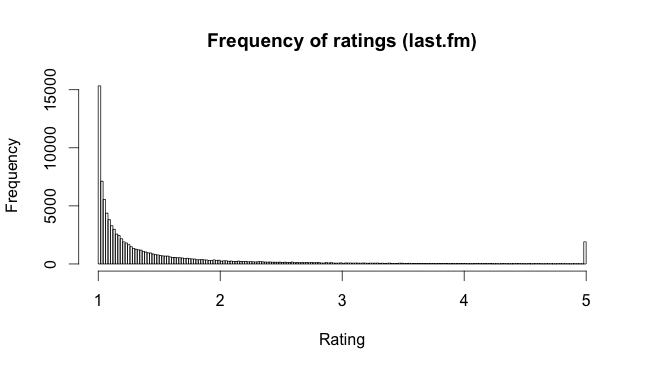
\includegraphics[width=425px]{./3-artificialdata/figures/FrequencyOfRatings_Lastfm.png}
\label{f:frequencyofratings}
\caption{Frequency of ratings of the last.fm dataset}
\end{figure}

Since it is assumed and to be shown that there exists a certain correlation between friends' ratings, this also has to be included in the rating generation. Varying the degree of correlation will help to show if social network information can increase collaborative filtering performance.

\section{k-fold Cross-Validation}
\label{st:kfoldcrossvalidation} 